\documentclass[journal,twoside]{IEEEtran}
\usepackage{cite}
\usepackage{float}
\usepackage[pdftex]{graphicx}
\graphicspath{{./shuntactive/}}
\DeclareGraphicsExtensions{.pdf,.jpeg,.png,.jpg}
\usepackage{amsmath}
\usepackage{algorithmic}
\usepackage{array}
\usepackage{etoolbox}
\patchcmd{\thebibliography}{\section*{\refname}}{}{}{}
\patchcmd{\thebibliography}{\addcontentsline{toc}{section}{\refname}}{}{}{}
\usepackage{url}
    \begin{document}
    \setcounter{page}{9}
    \title{Design and Fabrication of a Shunt Active Power Filter for a 3 Phase 4 Wire System Using The P-Q Theory}
    \author{{Abhaya Singh Pandey, Abodh Poudyal, Ashuhang Rai and Deepak Joshi}\\
 \IEEEauthorblockA{Department of Electrical Engineering,\\
 Institute of Engineering, Pulchowk, Lalitpur} }

\markboth{Zerone Scholar,~Vol.~1, No.~1, November~2016}%
{Pandey \MakeLowercase{\textit{et al.}}: Shunt Active Power Filter}

\maketitle

\begin{abstract}
This paper presents the basic operating principle of a Shunt Active Power Filter (SAPF) for a 3 phase 4 wire system. Shunt active power filters are widely employed for the compensation of harmonic currents, reactive power and elimination of unbalanced currents. A MATLAB model has also been presented in this paper along with the results to verify the compensating action of SAPF.
\end{abstract}


	\begin{IEEEkeywords}
Harmonics, Inverter, Non-linear loads, PI controller, Reactive Power, Shunt active power filter 
	\end{IEEEkeywords}


	\section{Introduction}
Development in the field of semiconductor devices and power electronics has resulted in an increased use of non-linear devices and circuits which results in complex problems and losses in power system networks. In simple words, non
linear loads are those types of loads which do not draw sinusoidal currents from the source while their counterparts,
linear loads draw currents which are more or less perfectly sinusoidal. The voltage-current relationship of non-linear loads
is not linear and while these devices perform complex operations in an efficient way but they pose certain problems
in a power system network which cannot be entirely ignored. A common example of a non linear device is a diode
which does not exhibit a linear voltage-current relationship. A more practical example of a non-linear load is a rectifying
circuit with an inductive load which employs diodes or thyristors for conversion of ac power into dc power for various
purposes. A rectifying circuit with an inductive load doesn’t draw sinusoidal current form the source. In fact, the waveform
of the current drawn by this circuit is almost of square wave in nature which is symmetrical about the ‘time’ axis.
Fourier analysis of the current waveform drawn by a non-linear load helps us to resolve the waveform into its sinusoidal
harmonic components and these harmonic components are undesirable in any power system network as they tend to
increase the losses in the system. They oscillate at frequencies which are integral multiples of the fundamental frequency and
can impose problems whose mitigation is very important in any power system network.
	

\section{Shunt Active Power Filter}
A shunt active power filter is designed to be connected across the non-linear load which ultimately mitigates the
problems related to the compensation of reactive power, harmonic currents and unbalanced current flowing through the
neutral wire in a three phase four wire system. The designed power filter operates on the basis of the
instantaneous power theory or the p-q theory which works on the basic idea of resolving the complex power into active and
reactive power and further resolving each of them into oscillating and non-oscillating parts.
The P-Q Theory or \lq\lq Instantaneous Power Theory\rq\rq was developed by Akagi et al in 1983, with the objective of
applying it to the control of active power filters. It is based on the instantaneous values of currents and voltages in three-
phase power systems with or without neutral wire and is valid for steady-state or transient operations. The P-Q theory consists
of an algebraic transformation (Clarke transformation) of the three-phase voltages and currents in the a-b-c coordinates into
$\alpha - \beta - 0$ coordinates followed by the calculation of the instantaneous power components.
The equations required for calculation of current and
voltage in $\alpha-\beta$ axes are given below along with the calculation
of instantaneous power. 


\[ \begin{bmatrix} v_0 \\ v_{\alpha} \\v_{\beta} \end{bmatrix}
=\sqrt{\frac{2}{3}} \begin{bmatrix} \frac{1}{\sqrt 2} & \frac{1}{\sqrt 2} &\frac{1}{\sqrt 2}\\ 1 & \frac{-1}{2} & \frac{-1}{2}\\ 0 & \frac{\sqrt 3}{2} & \frac{-\sqrt 3}{2} \end{bmatrix} \begin{bmatrix} v_a \\ v_b \\ v_c \end{bmatrix} \] 


\[ \begin{bmatrix} i_0 \\ i_{\alpha} \\i_{\beta} \end{bmatrix}
=\sqrt{\frac{2}{3}} \begin{bmatrix} \frac{1}{\sqrt 2} & \frac{1}{\sqrt 2} &\frac{1}{\sqrt 2}\\ 1 & \frac{-1}{2} & \frac{-1}{2}\\ 0 & \frac{\sqrt 3}{2} & \frac{-\sqrt 3}{2} \end{bmatrix} \begin{bmatrix} i_a \\ i_b \\ i_c \end{bmatrix} \] 


\[ \begin{bmatrix} p_0 \\ p \\q \end{bmatrix}
=\sqrt{\frac{2}{3}} \begin{bmatrix} v_0 & 0 &0\\ 0 & v_{\alpha} & v_{\beta}\\ 0 & -v_{\beta} & v_{\alpha} \end{bmatrix} \begin{bmatrix} i_0 \\ i_{\alpha} \\ i_{\beta} \end{bmatrix} \] 



After the necessary filtering and extraction of the oscillating
and non-oscillating parts, the compensating currents for the
three phases are calculated by the following equations.
\[\begin{bmatrix} {i_{\alpha}}^{ref}\\{i_{\beta}}^{ref} \end{bmatrix} = \frac{1}{v_{\alpha}^2+v_{\beta}^2} \begin{bmatrix} v_{\alpha} & -v_{\beta}\\v_{\beta} & v_{\alpha} \end{bmatrix} \begin{bmatrix} \tilde{p} +{\bar{p}_{loss}} \\ -q \end{bmatrix}
\]



\[ \begin{bmatrix} i_{ca} \\ i_{cb} \\i_{cc} \end{bmatrix}
=\sqrt{\frac{2}{3}} \begin{bmatrix} 1 & 0\\ \frac{-1}{2} & \frac{\sqrt 3}{2}\\ \frac{-1}{2} & \frac{-\sqrt 3}{2} \end{bmatrix} \begin{bmatrix} i_{\alpha} \\ i_{\beta} \end{bmatrix} \] 

A Hysteresis Band Controller is used to generate gate
pulses which are used to drive the MOSFETS in our inverter.
The gate pulses are generated by comparing the reference
current generated by the instantaneous P-Q calculations and
the current injected into the system.\\
To sum it up, SAPF is basically an alternative source that
provides the necessary oscillating power corresponding to the
harmonic current components drawn by the load. After its
operation, the source will be able to view the load as a
balanced resistive load instead of an unbalanced inductive
load. Since it can also compensate reactive component, it can
also be termed as a universal filter. SAPF consists of the
following major components.

\begin{figure}[!ht]
\centering
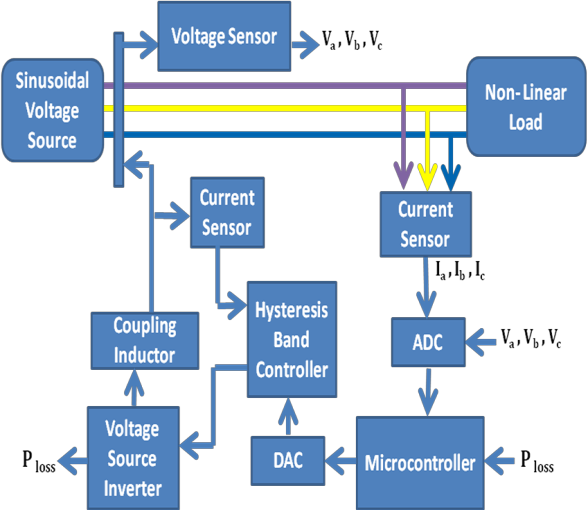
\includegraphics[width=3in]{1}
\caption{Schematics of a Shunt Active Power Filter}
\label{f1}
\end{figure}
\begin{itemize}
\item[A.] \emph{Reference current calculation block:}This block
consists of the equipments that sense the voltage and
current at Point of Common Coupling (PCC) and a programmed microcontroller to
calculate the Reference Current (current that is to be
compensated by the filter). This block uses IPS for
calculation of compensating current.
\item[B.]\emph{Source to inject compensating current: }The source is
a 3 phase inverter with a dc link of two capacitors
with enough capacity to store voltage for
compensation. The inverter output is controlled
according to gate pulses provided by controller. Since
the output of the inverter changes instantly to limit
the current change, the inverter terminal is connected
to PCC through coupling inductors.
\item[C.]\emph{Hysteresis band controller:} This is the gate sequence
generator for 3 phase inverter so that the capacitors
charge and discharge accordingly. It generates gate
pulses by comparing reference current with actual
current injected. If Raspberry Pi is used as
microcontroller, fabrication of a separate HBC circuit
is not necessary.
\item[D.]\emph{PI controller:} This controller generates the signal
P loss accordingly as the voltage level across capacitor
deviates from the specified value due to switching
losses in the inverter.
\end{itemize}

The basic schematic diagram of a shunt active power
filter is shown in fig~\ref{f1}.


\newpage
	\section{Simulation and Results}
Simulation of the SAPF was done in MATLAB and the
results were studied. Simulation was done with a line voltage
of 400 V and the SAPF was connected after 0.1 seconds. The
images of the simulation are shown in fig~\ref{a1},~\ref{a2}.
\begin{figure}[!ht]
\centering
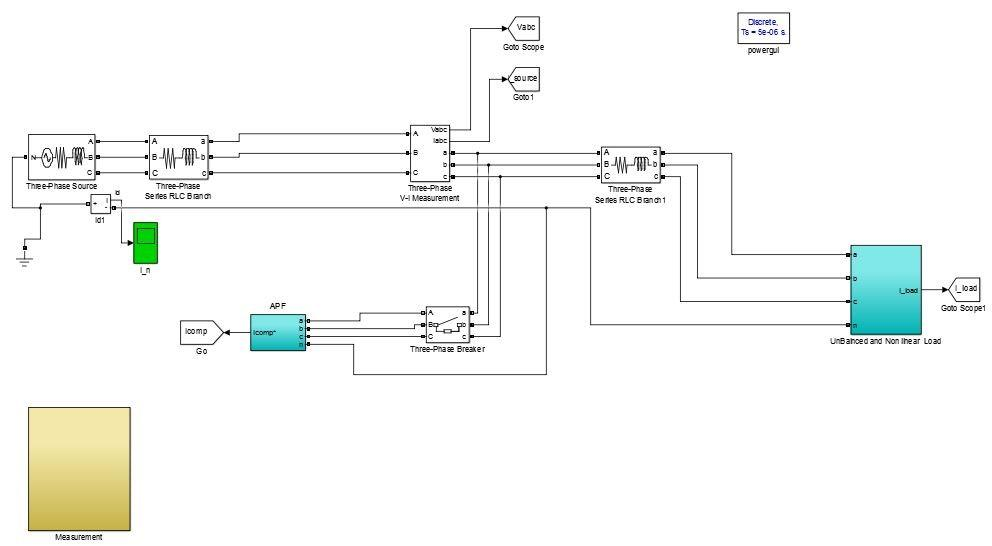
\includegraphics[height=3in , angle =90]{a1}
\caption{Overall System with Shunt Active Power Filter}
\label{a1}
\end{figure}

The results were obtained as expected and are shown in the figures~\ref{f2},~\ref{f3},~\ref{f4}
\begin{figure}[!htbp]
\centering
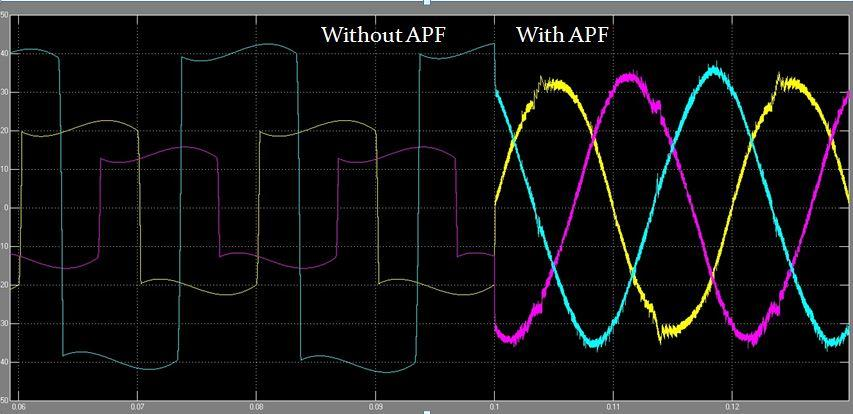
\includegraphics[width=3in]{2}
\caption{Graph of Source current Against time (SAPF is switched on at 0.1s)}
\label{f2}
\end{figure}

\begin{figure}[H]
\centering
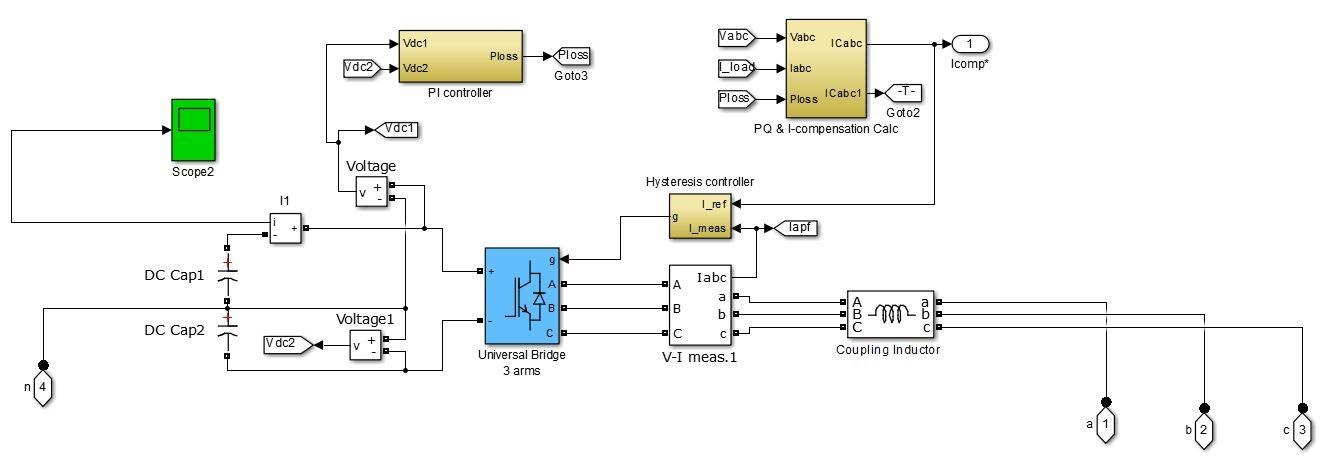
\includegraphics[height=3in, angle =90]{a2}
\caption{Shunt active power filter block}
\label{a2}
\end{figure}





\begin{figure}[!ht]
\centering
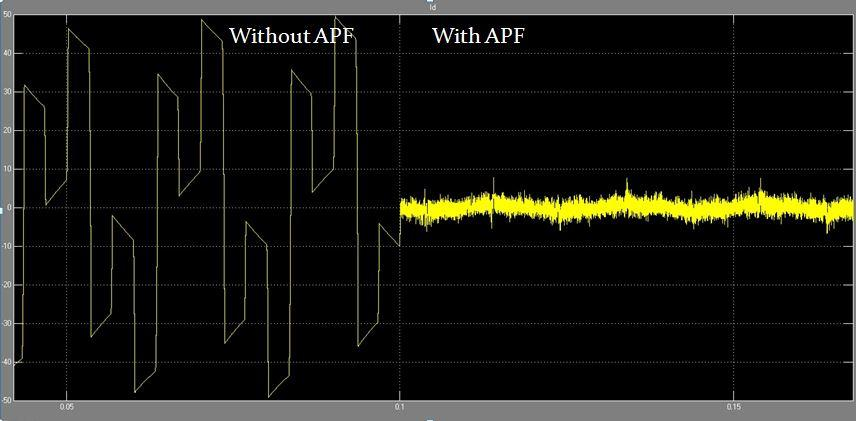
\includegraphics[width=3in]{3}
\caption{Graph of neutral current against time (SAPF is switched on at
0.1s)}
\label{f3}
\end{figure}

\begin{figure}[!ht]
\centering
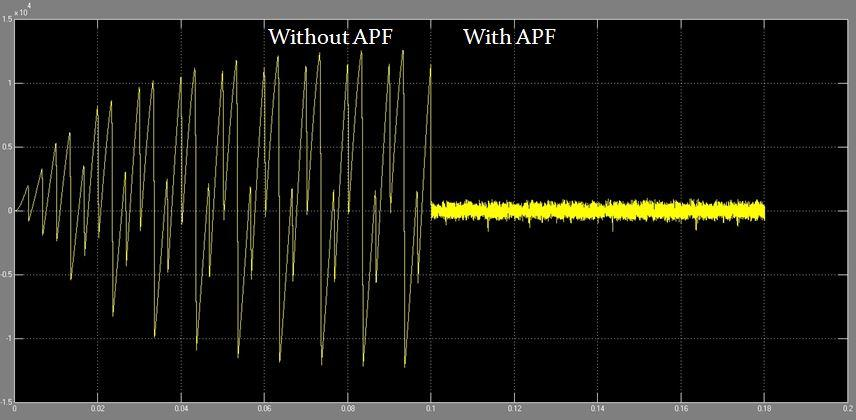
\includegraphics[width=3in]{4}
\caption{Graph of reactive power against time (SAPF is switched on at
0.1s)}
\label{f4}
\end{figure}


The THD of the load and the source current after the
operation of SAPF are shown in the table below.


\begin{table}[!ht]
\caption{THD of load and source currents after the operation of SAPF}
\label{t1}
\centering
\begin{tabular}{|c|c|c|c|}
\hline
Phase & A & B & C\\
\hline
Load Current THD & 43.91\% & 42.46\% & 44.25\%\\
\hline
Source Current THD & 4.88\% & 4.99\% & 4.22\%\\
\hline
\end{tabular}
\end{table}

\section{Hardware Components}
\subsection{Three Phase Inverter}
A three phase inverter is used to inject an approximated
version of the compensating current into the system at PCC.
The MOSFETS of the inverter are triggered according to the
gate pulses generated by the band controller.
\begin{figure}[!ht]
\centering
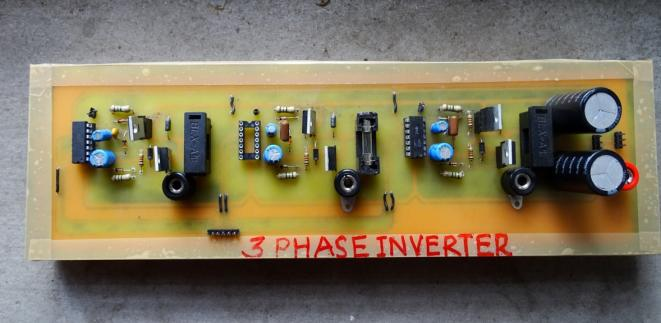
\includegraphics[width=3in]{5}
\caption{3 Phase Inverter}
\label{f5}
\end{figure}
\subsection{Voltage Sensor Circuit}
A voltage sensor circuit is required to sense the voltage at
PCC (Point of Common Coupling) and produce a de-amplified
version of the voltage. The output of the voltage sensor circuit
is then fed into the microcontroller for the calculation and
generation of compensating current.
\begin{figure}[!ht]
\centering
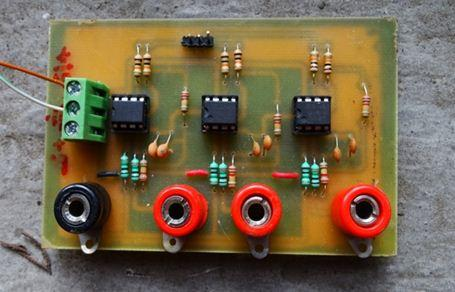
\includegraphics[width=3in]{6}
\caption{Voltage Sensor Circuit}
\label{f6}
\end{figure}
\subsection{Current Sensor Amplifier Circuit}
The current sensor produces an output voltage
corresponding to the current fed to it. The output should be
amplified before being fed into the microcontroller. An
amplifier circuit is therefore required in order to amplify the
output of the current sensor.
\begin{figure}[!ht]
\centering
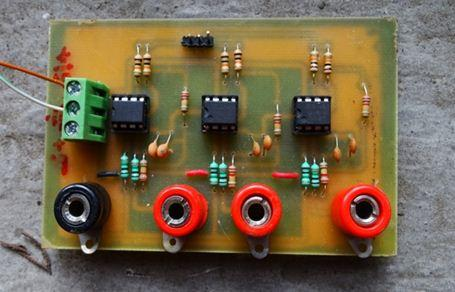
\includegraphics[width=3in]{6}
\caption{Current Sensor Amplifier Circuit}
\label{f6}
\end{figure}
\subsection{Three Phase Bridge Rectifier}
A three phase bridge rectifier is fabricated and is used
with three inductors to create a non-linear load that doesn't
draw sinusoidal current from the supply.
\begin{figure}[!ht]
\centering
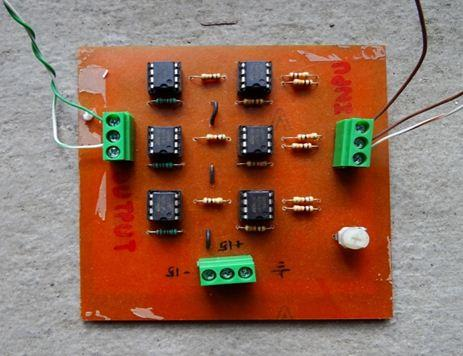
\includegraphics[width=3in]{7}
\caption{3 Phase Bridge Rectifier}
\label{f7}
\end{figure}

\section{Conclusion}
The three phase four wire shunt active filter with controller
based on Instantaneous Power Strategy is simulated in
MATLAB/SIMULINK to compensate the problems of the
harmonics and reactive power which are encountered from the
use of non-linear loads. The performance of the shunt active
power filter is investigated under different scenarios. It has
been observed that the P-Q theory based active filter manages
to compensate the harmonics, reactive power and neutral
current in a power distribution network. The active power
filter is able to reduce the THD in source current at a level
well below the international standards. The THD in source
current after employing the active filter is not exactly zero
because of the harmonics generated by the internal switching
of the compensator itself.


\section*{Bibliography}

\begin{thebibliography}{9}
    \bibitem{Akagi1983} 
        H. ~Akagi, Y. ~Kanazawa and A. ~Nabae, \lq\lq Generalized Theory of Instantaneous Reactive Power and Its Applications\rq\rq,\emph{ Transactions of the IEE-Japan}, Part B, Vol. 103, No.7, 1983, Pg 483-490 (In Japanese).
    \bibitem{Isabel2007} 
        Mar\'ia Isabel Milan\'es Montero, Enrique Romero Cadaval and Ferm\'in Barrero Gonz\'alez, \lq\lq Comparison of Control Strategies for Shunt Active PowerFilters in Three-Phase Four Wire Systems,\rq\rq\emph{ IEEE Transactions on Power Electronics}, Vol. 22, No. 1, January 2007
    \bibitem{Clarke1943} 
        E. ~Clarke, \emph{Circuit Analysis of A-C Power Systems, Vol. I-Symmetrical and
        Related Components}, Wiley, 1943.
    \bibitem{Ribeiro2013} 
        R. ~L. A. Ribeiro, T. O. A. Rocha, R. M. Sousa, E. C. dos Santos Jr. and A. M. N. Lima, \lq\lq A Robust DC-Link Voltage Control Strategy to Enhance the
        Performance of Shunt Active Power Filters without Harmonic Detection Schemes,\rq\rq \emph{ IEEE Transactions on Industrial Electronics}, 2013
    \bibitem{Singh1999} 
        B. Singh, ~K. Al-Haddad and Ambrish Chandra, \lq\lq A Review of
        Active Filters for Power Quality Improvement,\rq\rq\emph{ IEEE Transactions on
        Industrial Electronics}, Vol. 46, No. 5, October 1999
\end{thebibliography}
\newpage

\begin{IEEEbiography}[{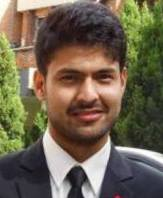
\includegraphics[width=1in,height=1.25in,clip,keepaspectratio]{asp}}]{Abhaya Singh Pandey} was born in August 22, 1993. He holds Bachelor in Electrical Engineering from Pulchowk Campus, IoE, Pulchowk. His fields of interest are Artificial Neural network, Automation, Power Electronics and Control System.
\end{IEEEbiography}

\vspace{-2cm}

\begin{IEEEbiography}[{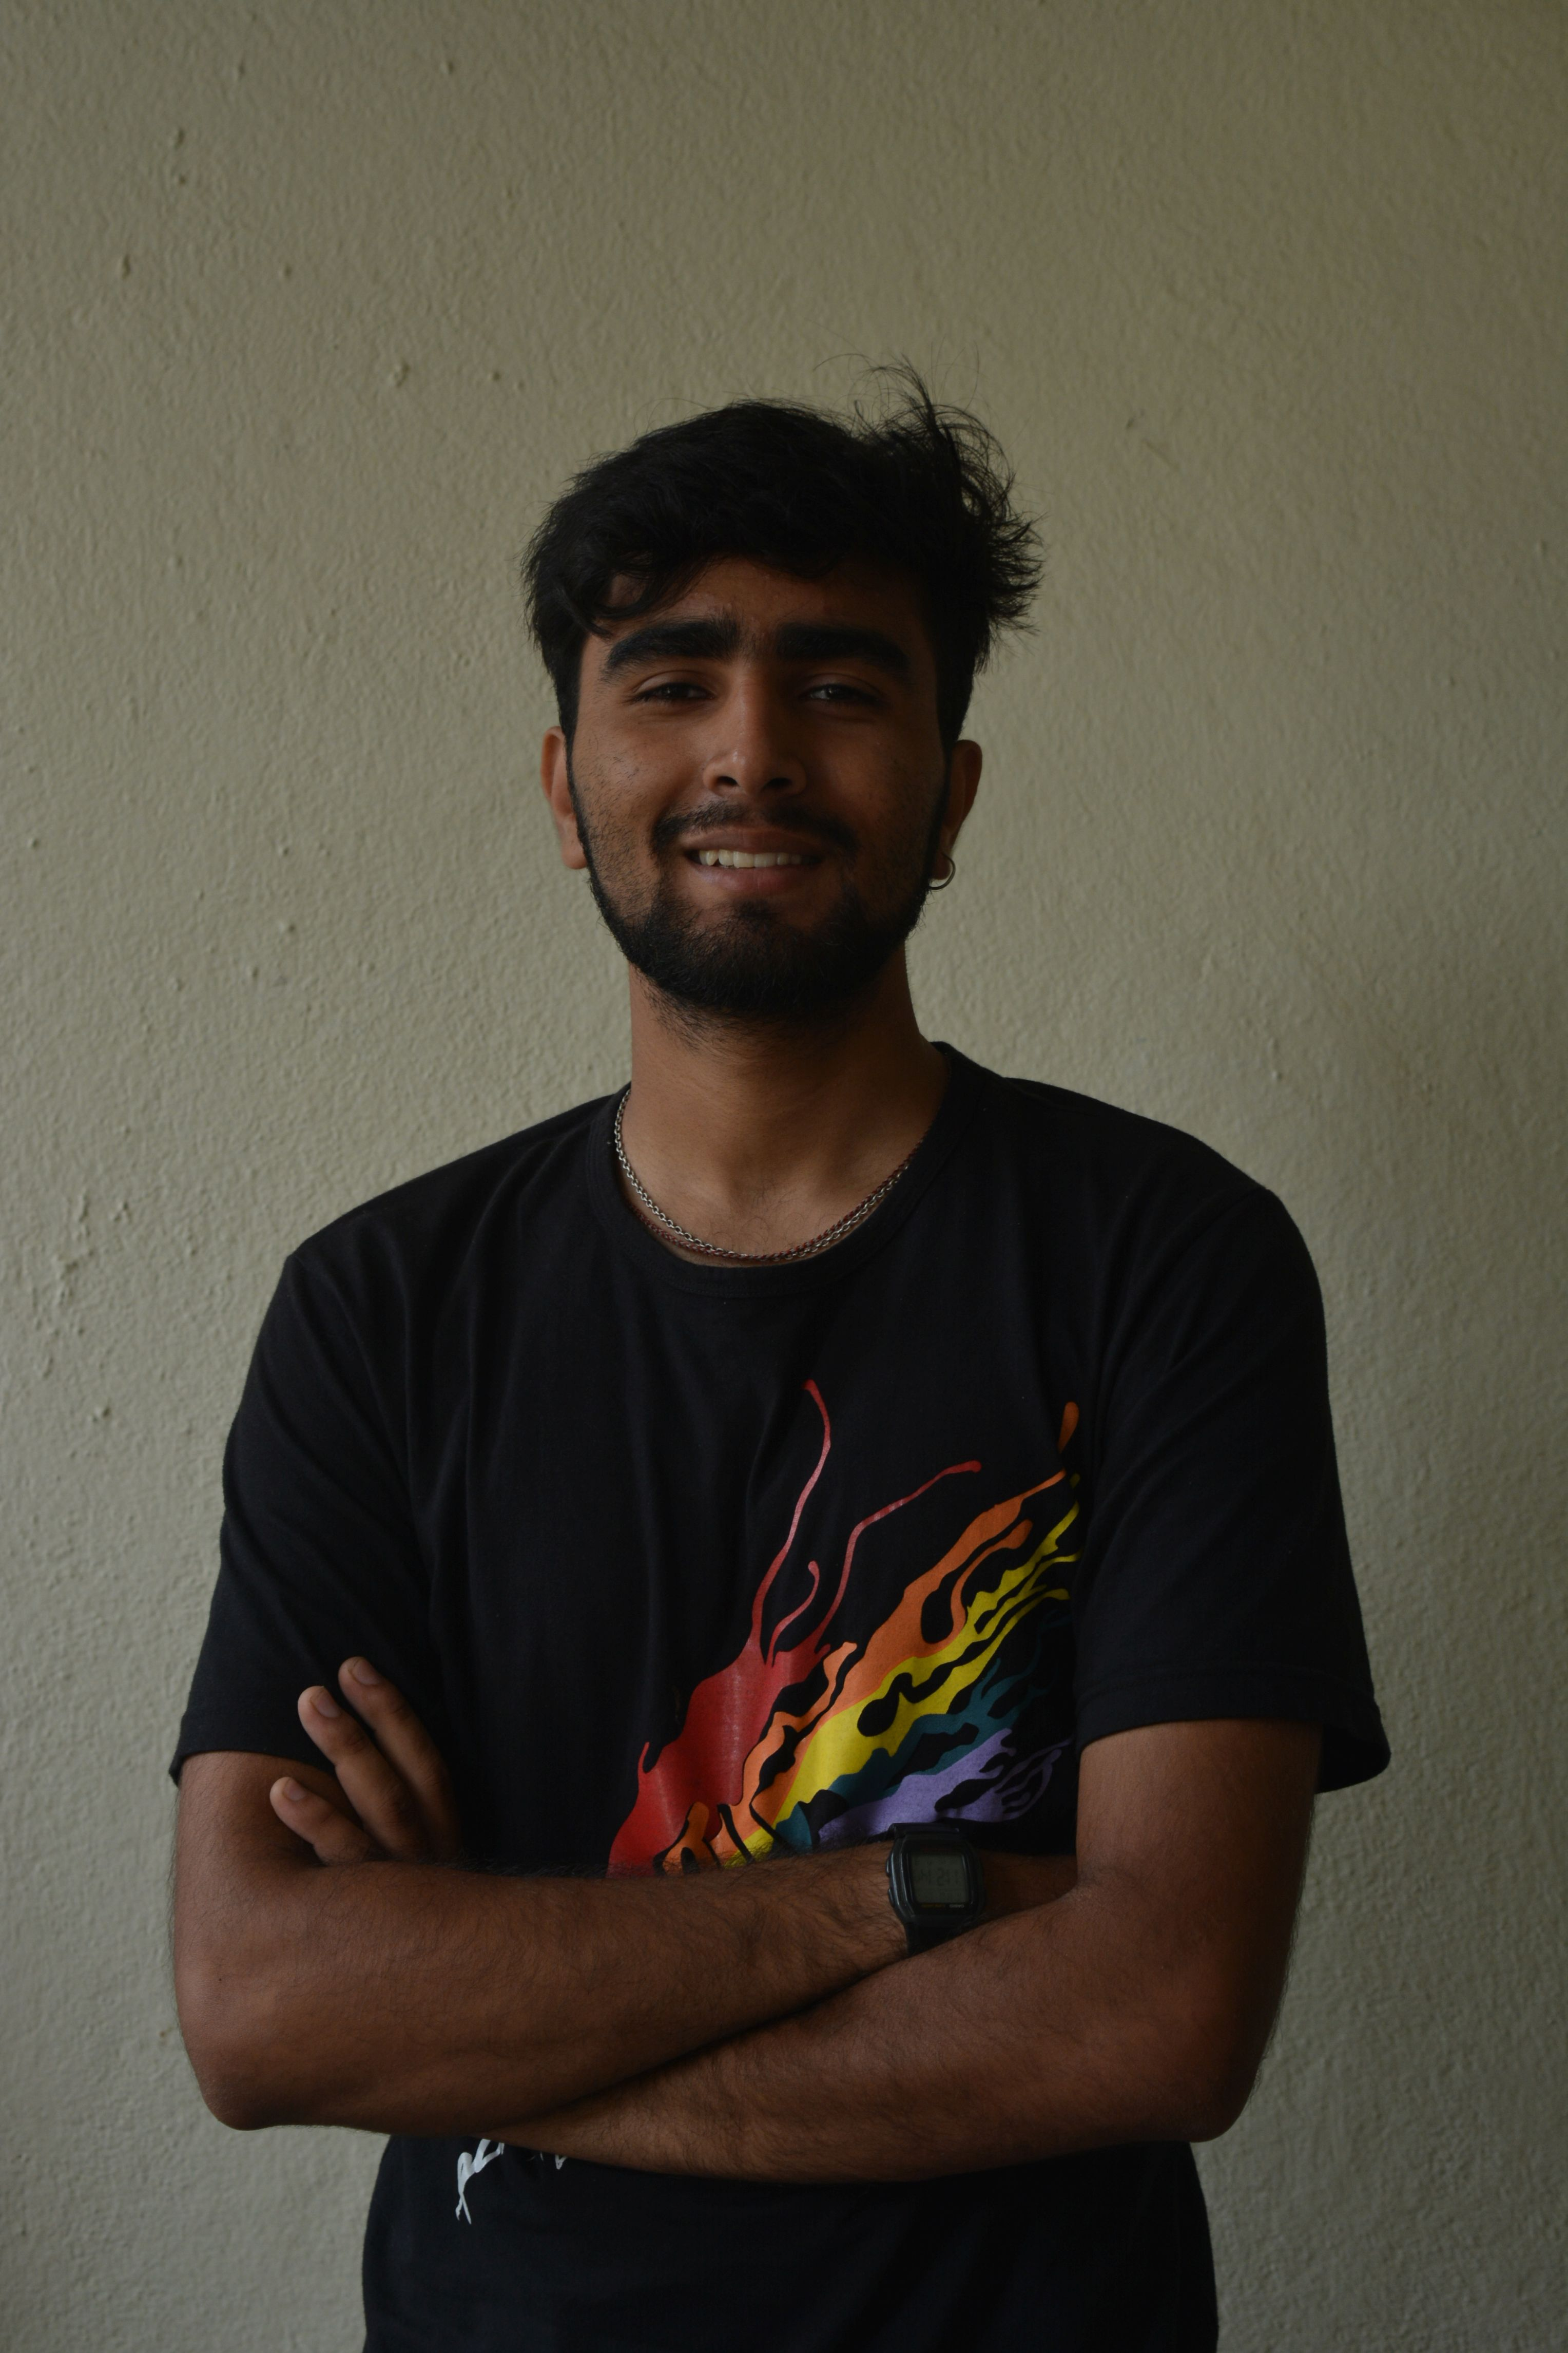
\includegraphics[width=1in,height=1.25in,clip,keepaspectratio]{ap}}]{Abodh Poudyal} was born in October 6, 1993. He holds Bachelor in Electrical Engineering from Pulchowk Campus, IoE, Tribhuvan University. His fields of interests are Power System, Power Electronics, Electrical Machine Drives and Control System.
\end{IEEEbiography}

\vspace{-2cm}

\begin{IEEEbiography}[{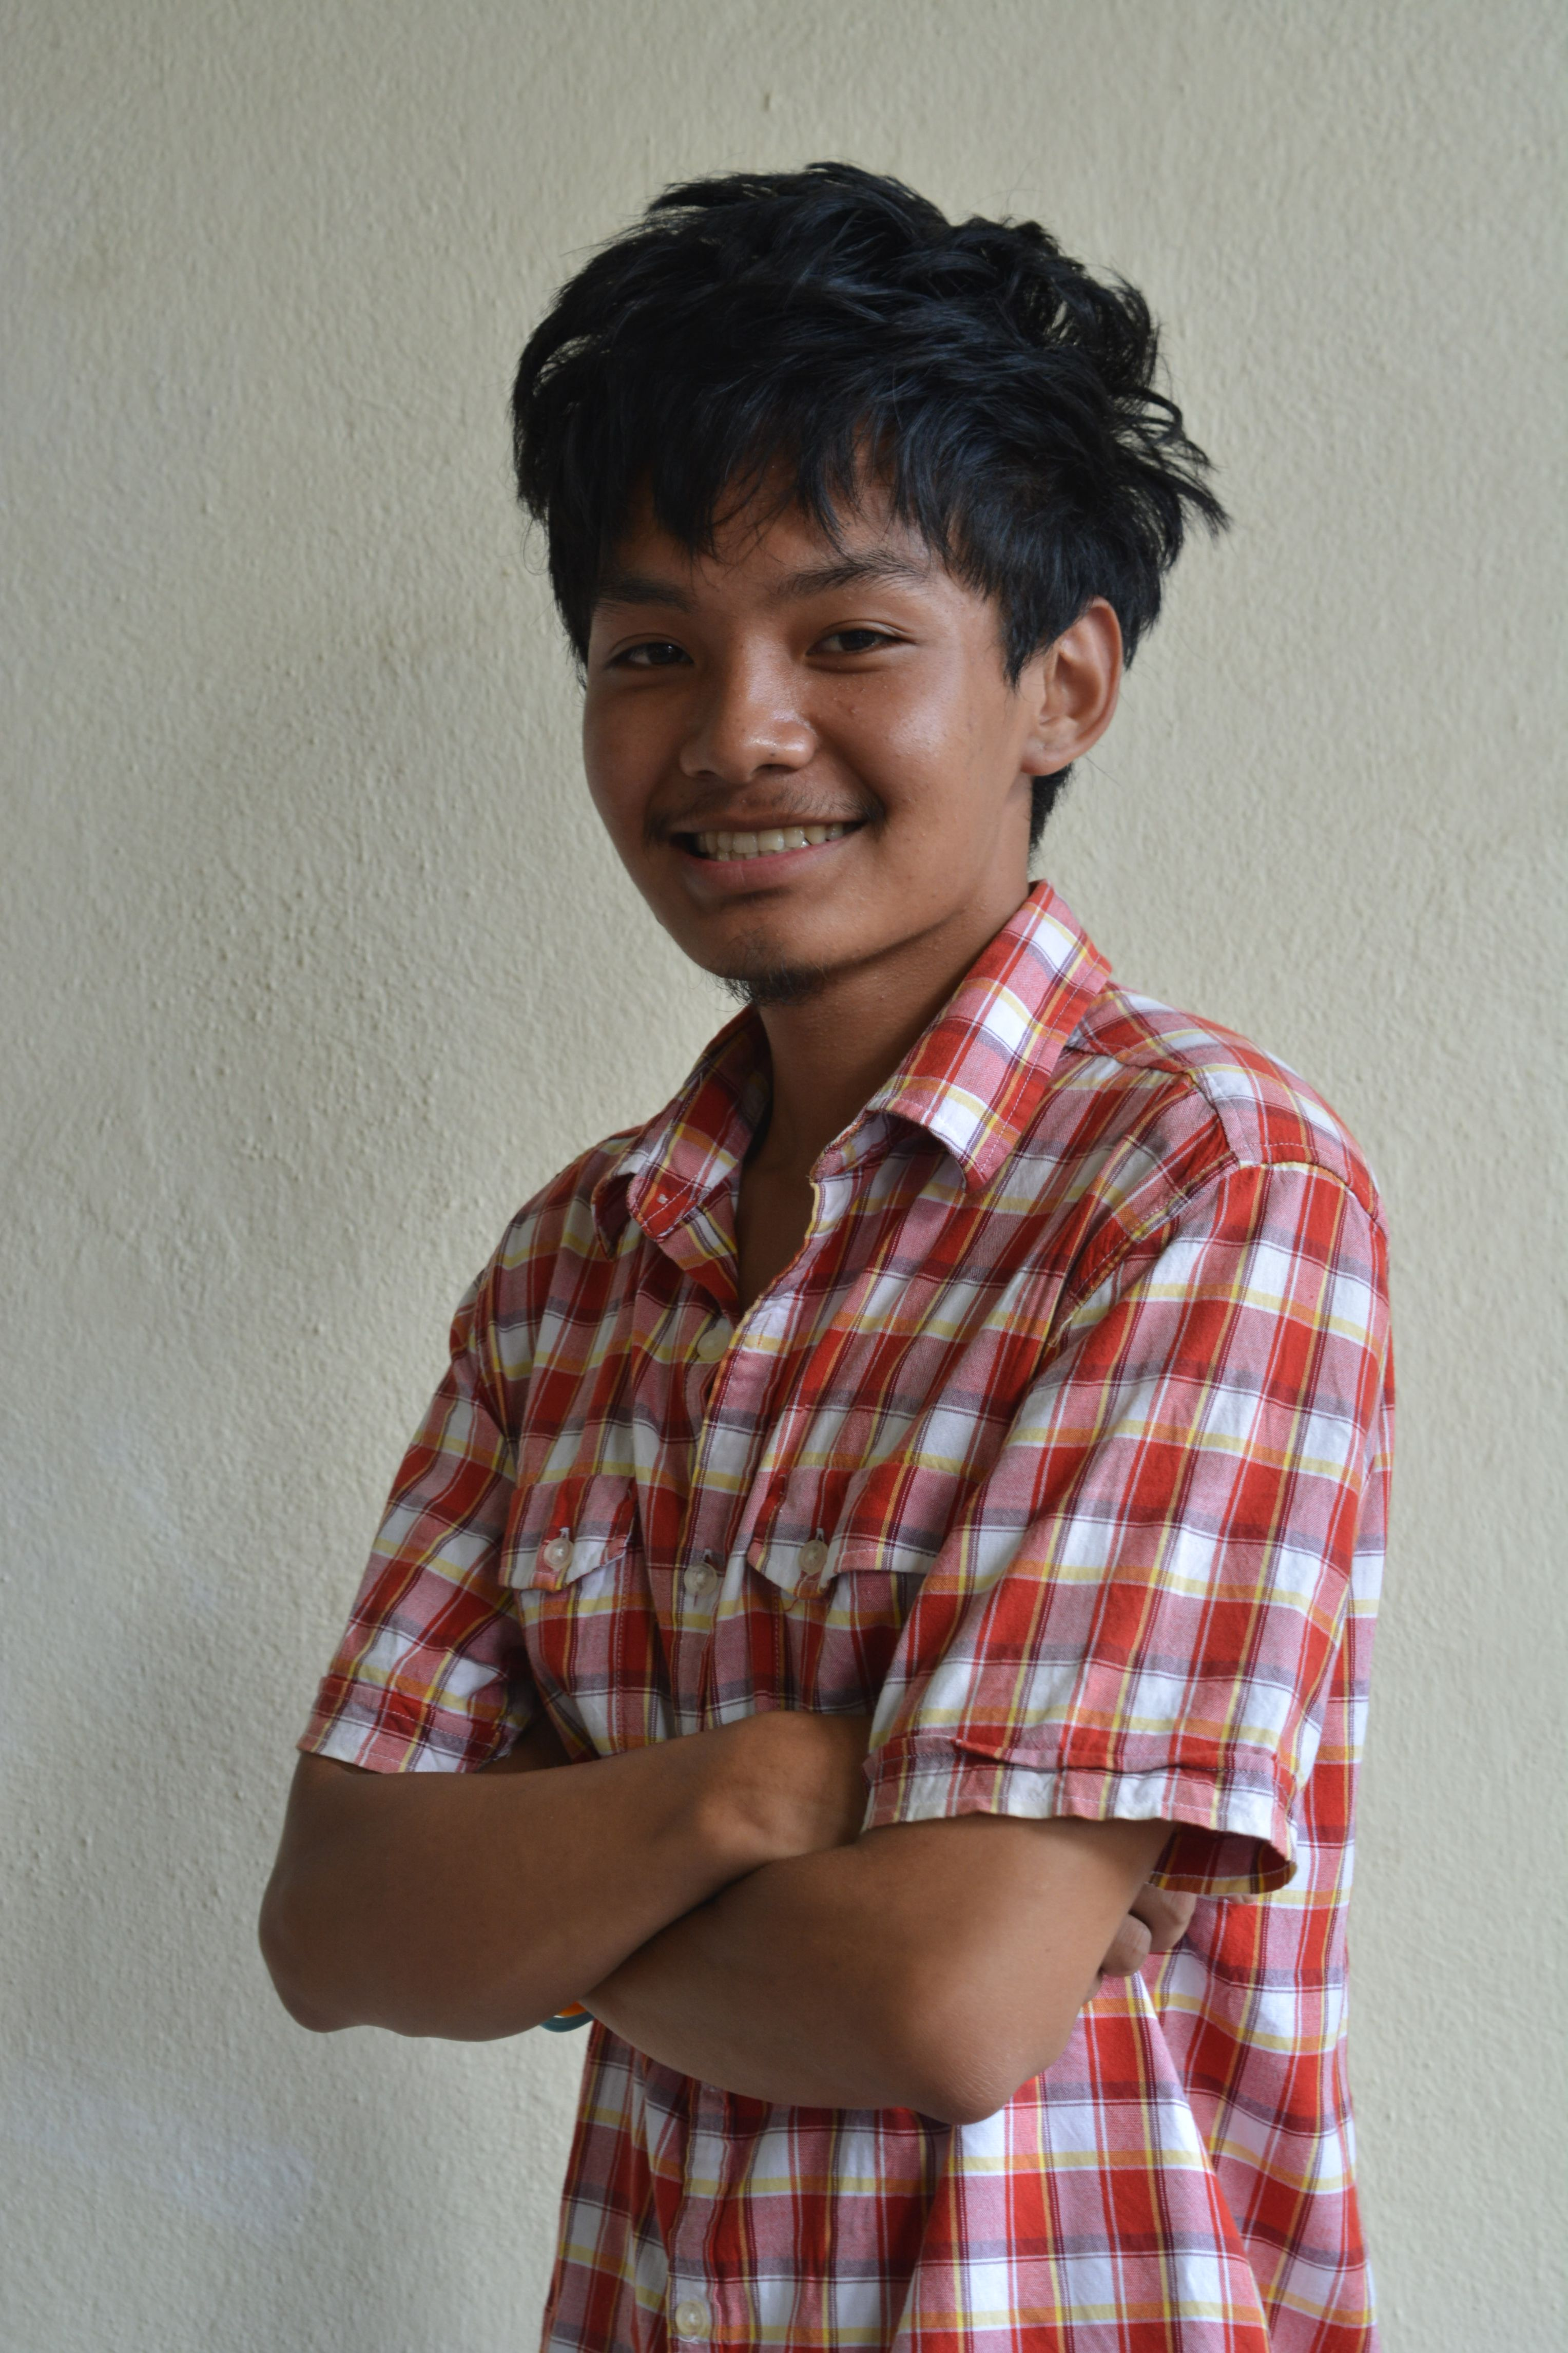
\includegraphics[width=1in,height=1.25in,clip,keepaspectratio]{ar}}]{Ashuhang Rai} was born in October 2, 1995.  He completed his Bachelor in Electrical Engineering from Pulchowk Campus, IoE, LAlitpur, Nepal. His research interest lies in the field of Power System, Power System Stability, Renewable Energy Sources Control and Rural Electrification.
\end{IEEEbiography}

\vspace{-2cm}

\begin{IEEEbiography}[{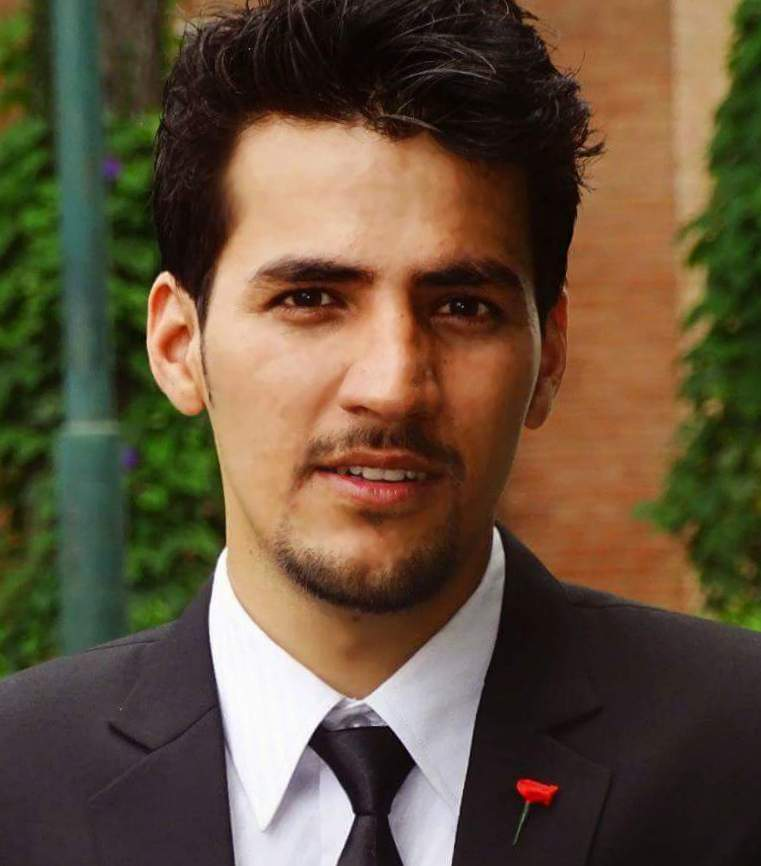
\includegraphics[width=1in,height=1.25in,clip,keepaspectratio]{dj}}]{Deepak Joshi} was born in July 10, 1994. He holds Bachelor in Electrical Engineering from Pulchowk Campus, IoE, Pulchowk. He is an enthusiast on Power Electronics, Power System, Electrical Machine Drives and Control System.
\end{IEEEbiography}




\end{document}

